\documentclass{../../../oss-apphys-exam}
\newcounter{last}

\begin{document}
%\genheader
\gentitle{6}{MAGNETISM, PART 1}

\raggedcolumns

\runningheader{
  \fontfamily{phv}\small
  \textcolor{gray}{AP PHYSICS C: ELECTRICITY AND MAGNETISM $\blacksquare$}
  \textbf{MULTIPLE-CHOICE QUESTIONS}}{}{}

\begin{multicols*}{2}
  \begin{questions}
    \question An electron is moving downward toward the bottom of the page when
    it passes through a region of magnetic field, as shown in the figure by
    the shaded area. The electron travels along a path that takes it through
    the spot marked $X$. The gravitational force on the electron is very
    small. What is the direction of the magnetic field?
    \begin{center}
      \begin{tikzpicture}[thick]
        \draw[dashed,fill=gray!20] circle (1);
        \node at (1.1,-.6) {$X$};
        \draw (0,2.5) circle (.1) node[above=3]{$e^-$};
        \draw[axes] (0,2.4)--(0,1);
      \end{tikzpicture}
    \end{center}
    \begin{choices}
      \choice Toward the bottom of the page
      \choice Toward the top of the page
      \choice Out of the page
      \choice Into the page
    \end{choices}
    
    \question Two long parallel wires carry currents ($I_A$ and $I_B$), as shown
    in the figure. Current $I_A$ in the left wire is twice that of current
    $I_B$ in the right wire. The magnetic force on the right wire is $F$. What
    is the magnetic force on the left wire in terms of $F$?
    \begin{center}
      \begin{tikzpicture}[scale=1.3,thick]
        \draw rectangle (.15,2);
        \draw (1,0) rectangle (1.15,2);
        \draw[axes] (.075,2)--(.075,3) node[above]{$I_A$};
        \draw[axes] (1.075,2)--(1.075,3) node[above]{$I_B$};
      \end{tikzpicture}
    \end{center}
    \begin{choices}
      \choice $F$ in the same direction
      \choice $F$ in the opposite direction
      \choice $F/2$ in the same direction
      \choice $F/2$ in the opposite direction
    \end{choices}
    \columnbreak
    
%    \question The figure below shows the microscopic dipoles inside two metal
%    objects. Copper is diamagnetic. Iron is ferromagnetic. Which of the
%    following best depicts the microscopic internal dipole position when the
%    objects are placed in a strong, external magnetic field directed toward the
%    top of the page?
%    \begin{center}
%      \pic{.15}{copper-iron}
%
%      \pic{.45}{domains}
%    \end{center}
%    \columnbreak
    
    \question A magnetic field, directed into the page, is placed between two
    charged capacitor plates, as shown in the figure. The magnetic and electric
    fields are adjusted so a proton moving at a velocity of $v$ will pass
    straight through the fields. The speed of the proton is doubled to $2v$.
    Which of the following force diagrams most accurately depicts the forces
    acting on the proton when traveling at $2v$?
    \begin{center}
      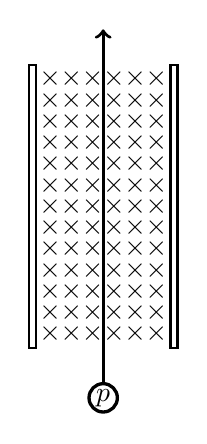
\begin{tikzpicture}[scale=.9]
        \begin{scope}[thick]
          \draw rectangle (.1,4);
          \draw(2,0) rectangle (2.1,4);
          \foreach\x in {.3,.6,...,2}{
            \foreach\y in {.2,.5,...,4} \node at (\x,\y) {$\times$};
          }
          \draw[very thick,->] (1.05,-.5)--(1.05,4.5);
          \draw[very thick] (1.05,-.7) circle (.2) node{$p$};
        \end{scope}
      \end{tikzpicture}
    \end{center}
    \begin{choices}
      \choice
      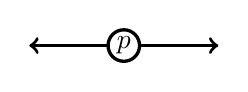
\begin{tikzpicture}[very thick]
        \draw circle (.2) node{$p$};
        \draw[->] (.2,0)--(1.2,0);
        \draw[->] (-.2,0)--(-1.2,0);
      \end{tikzpicture}
      
      \choice
      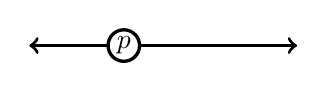
\begin{tikzpicture}[very thick]
        \draw circle (.2) node{$p$};
        \draw[->] (.2,0)--(2.2,0);
        \draw[->] (-.2,0)--(-1.2,0);
      \end{tikzpicture}

      \choice
      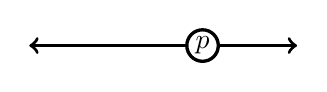
\begin{tikzpicture}[very thick]
        \draw circle (.2) node{$p$};
        \draw[->] (.2,0)--(1.2,0);
        \draw[->] (-.2,0)--(-2.2,0);
      \end{tikzpicture}
      
      \choice
      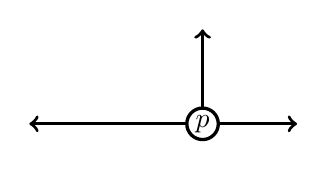
\begin{tikzpicture}[very thick]
        \draw circle (.2) node{$p$};
        \draw[->] (.2,0)--(1.2,0);
        \draw[->] (-.2,0)--(-2.2,0);
        \draw[->] (0,.2)--(0,1.2);
      \end{tikzpicture}
    \end{choices}
    \vspace{.7in}
    
    \question Which of the following is true concerning the force on the
    current-carrying wire due to the electron?
    \begin{center}
      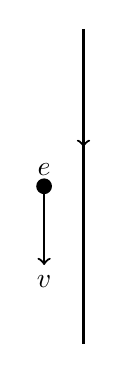
\begin{tikzpicture}[thick]
        \draw[->] (0,4)--(0,2.5);
        \draw (0,3)--(0,0);
        \fill(-.5,2) circle (.1) node[above] {$e$};
        \draw[->] (-.5,2)--(-.5,1) node[below]{$v$};
      \end{tikzpicture}
    \end{center}
    \begin{choices}
      \choice The force is directed toward the right.
      \choice The force is directed toward the left.
      \choice The force is directed into the page.
      \choice There is no force on the current-carrying wire due to the
      electron.
    \end{choices}
    \columnbreak
    
%    \question A loop of wire in the plane of the page carries a clockwise
%    current $I$ and is placed in a magnetic field that is directed into the
%    page as shown. Which of the following will happen as a result of the wire
%    loop being in the magnetic field?
%    \begin{center}
%      \begin{tikzpicture}
%        \foreach \x in {-1,0,1}{
%          \foreach \y in {-1,0,1}{
%            \node at (\x,\y) {$\times$};
%          }
%        }
%        \draw[thick] circle (.75);
%        \draw[thick,->] (-.75,0) arc(180:135:.75) node[above]{$I$};
%        \node at (1.3,1) {$B$};
%      \end{tikzpicture}
%    \end{center}
%    \begin{choices}
%      \choice The wire loop will rotate clockwise.
%      \choice The wire loop will rotate counterclockwise.
%      \choice The wire loop will flip on a horizontal axis through its center.
%      \choice The wire loop will expand in size.
%      \choice The wire loop will contract in size.
%    \end{choices}
%    
%    \uplevel{
%      \textbf{Questions \ref{q:2wires1}--\ref{q:2wires2}}
%  
%      Two wires carry currents $2A$ and $4A$ in the directions shown. Point $P$
%      is a distance $r$ from the wire carrying $2A$, and a distance $2r$ from
%      the wire carrying $4A$.
%      \begin{center}
%        \begin{tikzpicture}[scale=1.3]
%          \draw[thick] (0,0)--(2,0);
%          \draw[thick,->] (0,0)--(1.5,0) node[below]{$4A$};
%          \draw[thick] (0,0)--(0,2.5);
%          \draw[thick,->] (0,0)--(0,1.75) node[left]{$2A$};
%          \draw[thick,dashed] (0,2)--(1,2)node[midway,above]{$r$}
%          --(1,0) node[midway,right]{$2r$};
%          \fill (1,2) circle (.05) node[above right]{$P$};
%        \end{tikzpicture}
%      \end{center}
%    }
%
%    \question Which of the following statements is true?
%    \begin{choices}
%      \choice The magnetic field produced at point $P$ by the wire carrying
%      $2A$ is greater than the magnetic field produced at point $P$ by the wire
%      carrying $4A$, but opposite in direction.
%      \choice The magnetic field produced at point $P$ by the wire carrying
%      $2A$ is less than the magnetic field produced at point $P$ by the wire
%      carrying $4A$, and in the same direction.
%      \choice The magnetic field produced at point $P$ by the wire carrying
%      $2A$ is equal to the magnetic field produced at point $P$ by the wire
%      carrying $4A$, but opposite in direction.
%      \choice The magnetic field produced at point $P$ by the wire carrying
%      $2A$ is equal to the magnetic field produced at point $P$ by the wire
%      carrying $4A$, and in the same direction.
%      \choice The magnetic field produced at point $P$ by the wire carrying
%      $2A$ is greater than the magnetic field produced at point $P$ by the wire
%      carrying $4A$, and in the same direction.
%    \end{choices}
%    \label{q:2wires1}
%    \vspace{.7in}
%    
%    \question The magnitude of the resultant magnetic field at point $P$ due to
%    the current in the two wires is
%    \begin{choices}
%      \choice zero
%      \choice $\dfrac{\mu_0(2A)}{2\pi r}$
%      \choice $\dfrac{\mu_0(2A)}{\pi r}$
%      \choice $\dfrac{\mu_0(4A)}{2\pi r}$
%      \choice $\dfrac{\mu_0(6A)}{4\pi r}$
%    \end{choices}
%    \label{q:2wires2}

    \uplevel{
      \textbf{Questions \ref{q:2curr1}--\ref{q:2curr2}}: Two wires are parallel
      to each other, one carrying twice the current as the other. The two
      currents flow in the same direction.
    }

    \question Which of the following is true of the forces the wires exert on
    each other?
    \begin{choices}
      \choice The wire with the larger current exerts a greater force on the
      other wire.
      \choice The wire with the smaller current exerts a greater force on the
      other wire.
      \choice The wires exert equal and opposite forces on each other.
      \choice The wires exert equal forces on each other, but in the same
      direction.
      \choice The net force between the wires is zero.
    \end{choices}
    \label{q:2curr1}
    \vspace{.7in}
    
    \question The direction of the force between the wires is
    \begin{choices}
      \choice repulsive
      \choice attractive
      \choice zero
      \choice into the page
      \choice out of the page
    \end{choices}
    \label{q:2curr2}
    \vspace{.7in}
    
    %\question A dynamic microphone contains a magnet and a coil of wire
    %connected to a movable diaphragm, as shown in the figure. Sound waves
    %directed at the diaphragm generate a current in the wires leading from the
    %coil. Which of the following helps to explain why this occurs?
    %\cpic{.3}{mic}
    %\begin{choices}
    %  \choice The area of the coil changes.
    %  \choice The magnitude of the magnetic field produced by the magnet
    %  changes.
    %  \choice The angle between the plane of the coil and the magnetic field
    %  produced by the magnet change.
    %  \choice The strength of the magnetic field in the plane of the coil
    %  changes.
    %\end{choices}
    \columnbreak
    
    \uplevel{
      \textbf{Questions \ref{q:circ1}--\ref{q:circ2}}:
      A negatively charged particle of mass $m$ and charge $q$ in a uniform
      magnetic field $B$ travels in a circular path of radius $r$.
      \begin{center}
        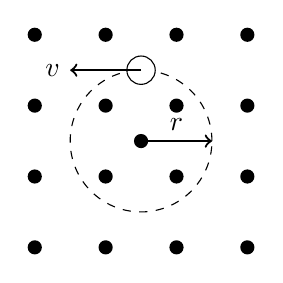
\begin{tikzpicture}[scale=.9]
          \foreach \x in {0,...,3}{
            \foreach \y in {0,...,3} \fill (\x,\y) circle (.1);
          }
          \fill (1.5,1.5) circle (.1);
          \draw[thick,->] (1.5,1.5)--(2.5,1.5) node[midway,above]{$r$};
          \draw[dashed] (1.5,1.5) circle (1);
          \draw[fill=white] (1.5,2.5) circle (.2);
          \draw[thick,->] (1.5,2.5)--(.5,2.5) node[left]{$v$};
        \end{tikzpicture}
      \end{center}
    }

    \question In terms of the other given quantities, the charge-to-mass ratio
    $q/m$ of the particle is
    \begin{choices}
      \choice $\dfrac{Bv}r$
      \choice $\dfrac r{Bv}$
      \choice $\dfrac{rv}B$
      \choice $rvB$
      \choice $\dfrac v{rB}$
    \end{choices}
    \label{q:circ1}
    
    \question The work done by the magnetic field after two full revolutions of
    the charge is
    \begin{choices}
      \choice zero
      \choice $-\dfrac{qv B}{rm}$
      \choice $\dfrac{qv m}{Br}$
      \choice $-\dfrac{mBr}{qv}$
      \choice $-mqv Br$
    \end{choices}
    \label{q:circ2}
    
%    \question A current is passed through an analog ammeter and the needle moves
%    to indicate the current flowing through the circuit. Which of the
%    following best explains how an analog ammeter works?
%    \begin{choices}
%      \choice Current is passed through the needle placed in a magnetic field,
%      and the needle is attracted to the high side of the scale.
%      \choice The needle is a magnet, and is attracted to a magnet on the high
%      side of the scale.
%      \choice The needle gathers an electrostatic charge from the current, and
%      is attracted to an electrostatic charge on the high side of the scale.
%      \choice Current is passed through a spring coil of wire placed in a
%      magnetic field, and the coil rotates, moving the needle
%      proportionally to the current in the coil.
%      \choice Current flows through the needle, making it heavier, and it falls
%      to the high side of the scale.
%    \end{choices}
%    \vspace{.7in}
%    
%    \question An electric motor consists of a current-carrying loop of wire
%    mounted to an axle and turned at a slight angle in a magnetic field as
%    shown. The wire loop will
%    \cpic{.35}{motor-drawing}
%    \begin{choices}
%      \choice experience a torque and turn clockwise
%      \choice experience a torque and turn counterclockwise
%      \choice accelerate upward out of the magnetic field
%      \choice accelerate downward out of the magnetic field
%      \choice not experience a force or torque
%    \end{choices}
  \end{questions}
  \setcounter{last}{\value{question}}
\end{multicols*}
\newpage

\runningheader{
  \fontfamily{phv}\small
  \textcolor{gray}{AP PHYSICS C: ELECTRICITY AND MAGNETISM $\blacksquare$}
  \textbf{FREE-RESPONSE QUESTIONS}}{}{}




\begin{questions}
  \setcounter{question}{\value{last}}
  
  % TAKEN FROM 2001 AP PHYSICS C EXAM FREE-RESPONSE QUESTION E&M 3
  \uplevel{
    \centering
    \begin{tikzpicture}[american voltages,scale=1.2]
      \draw[line width=3] (-5,0)--(5,0);
      \draw[line width=3] (-2,1)--(2,1) node[midway,above]{$\ell$};
      \draw[thick] (-2,1)--(-2,2.5) node[midway,left]{$d$}
      to[battery1=$\mathcal E$] (2,2.5)--(2,1) node[midway,right]{$d$};
      \draw[<->] (-1,1)--(-1,0) node[midway,fill=white]{$r$};
      \draw[<-] (4.7,0) to[in=270,out=-80] (5.5,-.3) node[above]{Cable};
      \draw[<-] (1.7,1) to[in=180,out=-80] (3,.85)
      node[right]{Rod (mass $m$, resistance $R$)};
      \draw[<-] (1.5,2.5) to[in=270,out=90] (2.5,3)
      node[above]{Fixed Horizontal Wires};
    \end{tikzpicture}
  }
  
  \question The circuit shown above consists of a battery of emf $\mathcal E$
  in series with a rod of length $\ell$, mass $m$, and resistance $R$. The rod
  is suspended by vertical connecting wires of length $d$, and the horizontal
  wires that connect to the battery are fixed. All these wires have negligible
  mass and resistance. The rod is a distance $r$ above a conducting cable. The
  cable is very long and is located directly below and parallel to the rod.
  Earth's gravitational pull is toward the bottom of the page. Express all
  algebraic answers in terms of the given quantities and fundamental constants.
  \begin{parts}
    \part\textbf{Determine} the magnitude and direction of the current $I$ in
    the rod
    \vspace{\stretch1}
    
    \part\textbf{Indicate} which direction must there be a current in the cable
    in order to exert an upward force on the rod? \textbf{Justify} your answer.
    \vspace{\stretch1}
    
    \part With the proper current in the cable, the rod can be lifted up such
    that there is no tension in the connecting wires. \textbf{Determine} the
    minimum  current $I_c$ in the cable that satisfies this situation.
    \vspace{\stretch1}
    
    %\part Determine the magnitude of the magnetic flux through the circuit due
    %to the minimum current $I_c$ determined in part (c).
  \end{parts}
  \newpage

  \uplevel{
    \centering
    \begin{tikzpicture}[scale=1.2]
      \draw rectangle (5,.2);
      \draw (0,1.8) rectangle (5,2);
      \draw (-.75,0.2) rectangle (-2.5,1.8) node[midway]{\small Radioactive};
      \foreach \x in {.5,1,...,4.5}{
        \foreach \y in {.5,1,1.5} \draw (\x,\y) circle (.08);
      }
      \draw[dashed] (0,1)--(7,1);
      \draw[very thick,<->] (4.3,.2)--(4.3,1.8) node[pos=.7,left]{$d$};
      \foreach \xx in {-.5,5.5}{
        \draw[fill=gray!60] (\xx,1) circle (.1);
        \draw[vectors] (\xx+.2,1)--(\xx+1.2,1) node[midway,above]{$v$};
      }
      \draw (5.4,1.3) rectangle (5.6,2.5);
      \draw (5.4,0.7) rectangle (5.6,-.5);
    \end{tikzpicture}
  }

  \question A lead box containing radioactive materials that emit both
  electrons and positrons is placed near an apparatus consisting of an
  evacuated capacitor that is filled with a magnetic field, as shown in the
  figure above. Electrons that enter along the center line of the capacitor
  plates travel straight through (undeflected) with a velocity of
  $v=\SI{1.0e7}{\metre\per\second}$ and out the hole in the center of the
  apparatus on the right. The capacitor plates are separated by a distance of
  $d=\SI{.020}\metre$; each plate has an area of $A=\SI{1.0e-4}{\metre\squared}$
  and a potential difference of $\Delta V$. A uniform magnetic field of
  $B=\SI{0.030}\tesla$ is directed out of the page between the plates, as shown
  in the figure.
  \begin{parts}
    \part\textbf{Explain} why it is acceptable to neglect the effects of
    gravity on the electrons passing through the apparatus.
    \vspace{\stretch1}
    
    \part\textbf{Explain} why the electrons pass through the capacitor plates
    undeflected. Support your argument with an algebraic equation
    and an appropriately drawn force diagram.
    \label{passthrough}
    \vspace{\stretch1}
      
    \part Use your equation from part \textbf{B} to \textbf{calculate} the
    potential difference ($\Delta V$) between the capacitor plates.
    \vspace{\stretch1}
      
    \part\textbf{Indicate} which capacitor plate has the highest potential.
    \textbf{Justify} your reasoning making reference to the electric field.
    \vspace{\stretch1}
      
    \part\textbf{Calculate} the magnitude of the energy that is stored in the
    capacitor.
    \vspace{\stretch1}
    \newpage

    \uplevel{
      A positron enters the apparatus along the same path as the electrons
      from part \textbf{B}.
    }
    
    \part\textbf{Explain} why the positron, traveling at the same speed as the
    electrons, will also travel straight through the device undeflected.
    Support your argument with an equation.
    \vspace{\stretch1}
      
    \part A second positron enters the apparatus at a speed of $2v$.
    \textbf{Sketch} the path of the positron through the capacitor plates on the
    figure.
    \vspace{.5in}
    
    \uplevel{
      An electron exits the apparatus at a velocity of
      $v=\SI{1.0e7}{\metre\per\second}$ parallel to a long wire of a circuit,
      as shown in the figure. The distance between the electron and the wire is
      \SI1{\milli\metre}.
      \begin{center}
        \begin{tikzpicture}[american voltages,scale=1.2]
          \draw (0,-.5)--(0,1)--(4,1)--(4,-.5) to[battery1=$\mathcal E$] (2,-.5)
          to[R=$R$] (0,-.5);
          \draw[fill=gray!60] (1.5,1.3) circle (0.1);
          \draw[vectors] (1.7,1.3)--(2.7,1.3) node[midway,above]{$v$};
        \end{tikzpicture}
      \end{center}
    }
    \part\textbf{Calculate} the potential difference-to-resistance ratio of the
    circuit such that the electron will experience a force $F$ of
    \SI{1.3e-16}\newton.
    \vspace{\stretch1}      
      
    \part\textbf{Draw} a force vector on the figure to show the direction of the
    force on the electron.
    \vspace{1in}
  \end{parts}
  \newpage
  
  \uplevel{
    \cpic{.6}{long-cylinder}
  }
  \question A section of a long conducting cylinder with inner radius $a$ and
  outer radius $b$ carries a current $I_0$ that has a uniform current density,
  as shown in the figure above.
  \begin{parts}
    \part Using Amp\`{e}re's law, \textbf{derive} an expression for the
    magnitude of the magnetic field in the following regions as a function of
    the distance $r$ from the central axis.
    \begin{subparts}
      \subpart $r<a$
      \vspace{\stretch1}
      
      \subpart $a<r<b$
      \vspace{\stretch1}

      \subpart $r=2b$
      \vspace{\stretch1}
    \end{subparts}
    
    \part On the cross-sectional view in the diagram above, \textbf{indicate}
    the direction of the field at point $P$, which is at a distance $r=2b$ from
    the axis of the cylinder.
    \vspace{\stretch1}
    
    \part An electron is at rest at point $P$. \textbf{Describe} any
    electromagnetic forces acting on the electron. \textbf{Justify} your answer.
    \vspace{\stretch1}
    \newpage
    
    \uplevel{
      Now consider a long, solid conducting cylinder of radius $b$ carrying a
      current $I_0$. The magnitude of the magnetic field inside this cylinder
      as a function of $r$ is given by $B=\mu_0I_0r/2\pi b^2$. An experiment is
      conducted using a particular solid cylinder of radius \SI{.010}{\metre}
      carrying a current of \SI{25}\ampere. The magnetic field inside the
      cylinder is measured as a function of $r$, and the data is tabulated
      below.

      \vspace{.1in}
      \begin{center}
        \begin{tabular}{|l|l|l|l|l|l|}
          \hline
          Distance $r$ (m)    & 0.002 & 0.004 & 0.006 & 0.008 & 0.010\\ \hline
          Magnetic Field $B$ (T) & \num{1.2e-4} & \num{2.7e-4} & \num{3.6e-4}
          & \num{4.7e-4} & \num{6.4e-4} \\
          \hline
        \end{tabular}
      \end{center}
    }
    
    \part On the graph below, \textbf{plot} the data points for the magnetic
    field $B$ as a function of the distance $r$, and label the scale on both
    axes. \textbf{Draw} the best-fit line that best represents the data.
    \begin{center}
      \vspace{.4in}
      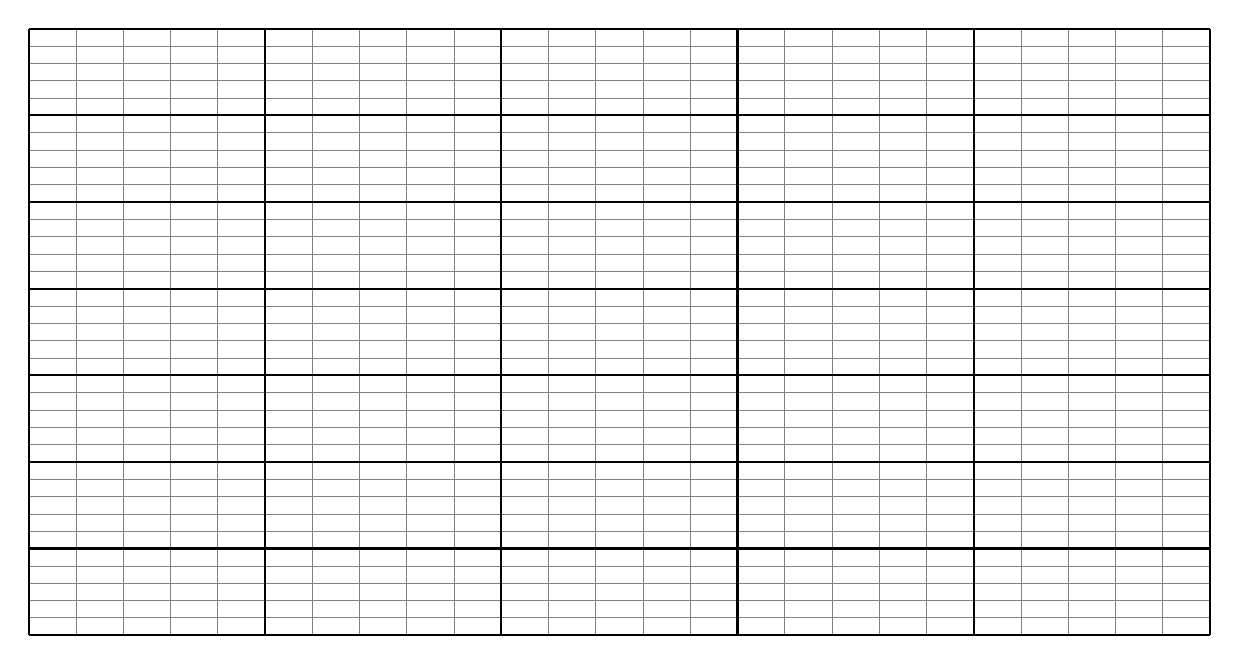
\begin{tikzpicture}[xscale=.6,yscale=.22]
        \draw[help lines] grid (25,35);
        \draw[thick,step=5] grid (25,35);
      \end{tikzpicture}
    \end{center}
    \vspace{.4in}

    \part Use the slope of your line to \textbf{estimate} a value of the vacuum
    permeability $\mu_0$.
  \end{parts}
\end{questions}
\end{document}
